\documentclass{exam-zh}

\usepackage{xeCJK}
\usepackage{background}
\usepackage{needspace}
\usepackage{listing}
\usepackage{setspace}

\examsetup{
  page = {
    foot-content = 「赴尘杯」思想政治试题第 ; 页(共 ; 页)
  }
}
\backgroundsetup{
  scale=20,
  color=black!10,
  opacity=1,
  angle=45,
  position=current page.center,
  contents={赴尘杯}
}

\newenvironment{kaiti-indented}{
  \parindent=2em
  \CJKfamily{zhkai}
  \setstretch{1.4}
}{
}

\title{2025 年陕西省高中学业水平选择性考试}
\subject[3.5em]{思想政治}

\begin{document}

\secret

\maketitle

本试卷共 16 页,67 题。全卷满分 150 分。考试用时 120 分钟。

\begin{notice}[][itemsep=0pt, parsep=0pt, topsep=0pt, partopsep=0pt]
\item 答卷前,考生务必将自己的姓名、准考证号填写在答题卡上。
\item 作答选择题时,选出每小题答案后,用 2B 铅笔在答题卡上对应题目选项的答案信息点涂黑,如需改动,用橡皮擦干净后,再选涂其他答案;作答非选择题时,用 0.5mm 黑色墨水签字笔在答题卡的对应题目位置作答,写在试题卷、草稿纸和答题卡上的非答题区域均无效。
\item 考试结束后,将本试卷和答题卡一并上交。
\end{notice}

\begin{flushleft}
  {\bfseries 一、选择题:本题共 16 小题,每小题 3 分,共 48 分。在每小题给出的四个选项中,只有一个选项是正确的。请将正确的选项填涂在答题卡相应的位置上。}
\end{flushleft}
\vspace{-1em}

\needspace{3\baselineskip}
\begin{question}
  习近平总书记在 2025 年新年贺词中指出:党的二十届三中全会胜利召开,吹响进一步全面深化改革的号角。我们乘着改革开放的时代大潮阔步前行,中国式现代化必将在改革开放中开辟更加广阔的前景。由此可见

  \circlednumber{1} 改革开放是决定当代中国命运的关键一招

  \circlednumber{2} 党的二十届三中全会标志着中国特色社会主义进入了新阶段

  \circlednumber{3} 全面深化改革有利于推进中国式现代化发展

  \circlednumber{4} 中国共产党坚持始终走在时代前列

  \begin{choices}
  \item \circlednumber{1}\circlednumber{2}
  \item \circlednumber{1}\circlednumber{3}
  \item \circlednumber{2}\circlednumber{3}
  \item \circlednumber{3}\circlednumber{4}
  \end{choices}
\end{question}

\needspace{3\baselineskip}
\begin{question}
  第二次世界大战后,资本主义有三大新变化:即新自由主义化、金融深化、全球经济虚拟化,这三大变化导致资本主义的不平等问题日益严重、经济出现停滞的趋势、泡沫经济和金融危机频发。由此可见

  \circlednumber{1} 资本主义政府难以实现经济宏观调控

  \circlednumber{2} 资本主义社会的基本矛盾是生产资料私有制和生产社会化的矛盾

  \circlednumber{3} 资本主义的不平等问题可能随着生产力的不断发展而得到解决

  \circlednumber{4} 周期性的资本主义经济危机是资本主义社会无法克服的障碍

  \begin{choices}
  \item \circlednumber{1}\circlednumber{2}
  \item \circlednumber{1}\circlednumber{4}
  \item \circlednumber{2}\circlednumber{3}
  \item \circlednumber{2}\circlednumber{4}
  \end{choices}
\end{question}

\needspace{3\baselineskip}
\begin{question}
  某校思想政治学习小组收集了我国不同时期领导人的经济论述。

  \begin{kaiti-indented}
    江泽民说:实践的发展和认识的深化,要求我们明确提出,我国经济体制改革的目标是建立社会主义市场经济体制,以利于进一步解放和发展生产力。

    胡锦涛说:提高开放水平,着力构建充满活力、富有效率、更加开放、有利于科学发展的体制机制,为发展中国特色社会主义提供强大动力和体制保障。

    习近平说:坚持和完善我国社会主义基本经济制度和分配制度,毫不动摇巩固和发展公有制经济,毫不动摇鼓励、支持、引导非公有制经济发展,使市场在资源配置中起决定性作用,更好发挥政府作用。
  \end{kaiti-indented}

  对以上论述的分析合理的是

  \circlednumber{1} 社会主义市场经济体制的建立和完善体现了党与时俱进的思想路线

  \circlednumber{2} 社会主义市场经济体制要求毫不动摇巩固公有制经济主体地位

  \circlednumber{3} 认识具有无限性,追求真理永无止境

  \circlednumber{4} 改革是社会主义社会实现社会变革的决定力量

  \begin{choices}
  \item \circlednumber{1}\circlednumber{3}
  \item \circlednumber{2}\circlednumber{3}
  \item \circlednumber{2}\circlednumber{4}
  \item \circlednumber{3}\circlednumber{4}
  \end{choices}
\end{question}

\needspace{3\baselineskip}
\begin{question}
  从党的十四届三中全会提出要建立社会保障制度,到党的十六大明确地把“社会保障体系比较健全”作为全面建设小康社会的目标之一,再到党的十八大把社会保障全民覆盖作为全面建成小康社会的重要目标,我国在推进社会保障制度建设的道路上行稳致远。以下说法合理的是

  \circlednumber{1} 社会保障是政府承担主要责任的“安全网”

  \circlednumber{2} 社会保障的运行方式是风险分摊和责任共担

  \circlednumber{3} 只有参与劳动的社会成员才有权享受社会保险提供的保障

  \circlednumber{4} 我国要最终建设覆盖全体人民的社会保障体系

  \begin{choices}
  \item \circlednumber{1}\circlednumber{2}
  \item \circlednumber{1}\circlednumber{3}
  \item \circlednumber{2}\circlednumber{3}
  \item \circlednumber{2}\circlednumber{4}
  \end{choices}
\end{question}

\needspace{3\baselineskip}
\begin{question}
  自 2025 年 1 月 1 日起各大银行将执行新的存量房贷利率,且绝大多数借款人不需要提交额外申请或办理相关手续。以贷款额 100 万元、等额本息、30 年期限为例,在房贷利率从 3.9\% 下调至 3.3\% 后,每月利息支出可节省 300 多元。由此可见

  \circlednumber{1} 中央人民政府通过调节财政政策刺激居民消费增长

  \circlednumber{2} 房贷利率随市场波动调节体现了市场在资源配置中的决定性作用

  \circlednumber{3} 中国人民银行积极促进金融业协调健康发展

  \circlednumber{4} 我国政府坚持把人民幸福作为发展的最终目的

  \begin{choices}
  \item \circlednumber{1}\circlednumber{2}
  \item \circlednumber{1}\circlednumber{3}
  \item \circlednumber{2}\circlednumber{3}
  \item \circlednumber{2}\circlednumber{4}
  \end{choices}
\end{question}

\needspace{3\baselineskip}
\begin{question}
  2024 年 12 月 26 日至 27 日,中共中央政治局召开民主生活会,会议上中央政治局的同志一致认为,以习近平同志为核心的党中央集中统一领导是做好一切工作的根本保证,确保中国式现代化航船乘风破浪、行稳致远,要坚持以习近平新时代中国特色社会主义思想为指导,坚持稳中求进工作总基调,扎实推动高质量发展,进一步全面深化改革,扩大高水平对外开放,保持社会和谐稳定。要求全体党员

  \circlednumber{1} 把锤炼党性、提高思想觉悟作为根本课题

  \circlednumber{2} 坚决维护以习近平同志为核心的党中央权威和集中统一领导

  \circlednumber{3} 坚持人民立场,打造人民满意的服务型政府

  \circlednumber{4} 始终走在时代前列,争做党和国家建设的先锋模范

  \begin{choices}
  \item \circlednumber{1}\circlednumber{2}
  \item \circlednumber{1}\circlednumber{3}
  \item \circlednumber{2}\circlednumber{3}
  \item \circlednumber{3}\circlednumber{4}
  \end{choices}
\end{question}

\needspace{3\baselineskip}
\begin{question}
  第十四届全国人民代表大会代表中,少数民族代表总数的 14.85\%,全国 55 个少数民族都有本民族的代表;妇女代表占代表总数的 26.54\%,提高了 1.64 个百分点;一线工人、农民代表占代表总数的 16.69\%,提高了 0.99 个百分点;专业技术人员占代表总数的 21.30\%,提高了 0.73 个百分点。由此可见

  \circlednumber{1} 全过程人民民主是最广泛的民主

  \circlednumber{2} 人民代表大会能够把人民意愿通过法律程序上升为国家意志

  \circlednumber{3} 我国的国体决定了人大代表的广泛性

  \circlednumber{4} 人民代表大会制度保障各领域、各阶层人民充分享有民主权利

  \begin{choices}
  \item \circlednumber{1}\circlednumber{3}
  \item \circlednumber{1}\circlednumber{4}
  \item \circlednumber{2}\circlednumber{3}
  \item \circlednumber{3}\circlednumber{4}
  \end{choices}
\end{question}

\needspace{3\baselineskip}
\begin{question}
  2024 年 12 月 12 日,中国国民党革命委员会第十四届中央委员会第三次全体会议在北京闭幕。全国政协副主席、民革中央常务副主席何报翔提出:要切实把思想和行动统一到中共中央决策部署上来,更好担当起中国共产党的好参谋、好帮手、好同事的政治责任。由此可见

  \circlednumber{1} 中国共产党领导各民主党派工作

  \circlednumber{2} 中国共产党领导的多党合作和政治协商制度是符合中国国情的新型政党制度

  \circlednumber{3} 人民政协始终坚持团结和民主为主题

  \circlednumber{4} 政协委员通过向人民代表大会提交提案履行参政权

  \begin{choices}
  \item \circlednumber{1}\circlednumber{3}
  \item \circlednumber{2}\circlednumber{3}
  \item \circlednumber{2}\circlednumber{4}
  \item \circlednumber{3}\circlednumber{4}
  \end{choices}
\end{question}

\needspace{3\baselineskip}
\begin{question}
  面对日益增长的环境问题,如何实现科学的、有质量的、可持续的发展成为新的时代课题。2005 年,时任浙江省委书记习近平创造性提出了“两山理论”:宁可不要金山银山也要绿水青山,因为绿水青山就是金山银山。党的十九大上,“两山理论”被写入党章。从中体现的哲学原理是

  \circlednumber{1} 同一事物的两个对立面既相互矛盾又辩证统一

  \circlednumber{2} 联系是客观的、普遍的,一切联系都以时间、地点和条件为转移

  \circlednumber{3} 认识没有终点,科学没有顶峰

  \circlednumber{4} 社会意识的变化发展可能影响社会存在的变化发展

  \begin{choices}
  \item \circlednumber{1}\circlednumber{2}
  \item \circlednumber{1}\circlednumber{4}
  \item \circlednumber{2}\circlednumber{3}
  \item \circlednumber{2}\circlednumber{4}
  \end{choices}
\end{question}

\needspace{3\baselineskip}
\begin{question}
  观察三幅夏季奥运会会徽,可得出的认识有

  \begin{multifigures}
    \item[1952 年芬兰奥运会] 
\includegraphics[width=5cm]{helsinki.png}
    \item[2008 年北京奥运会] 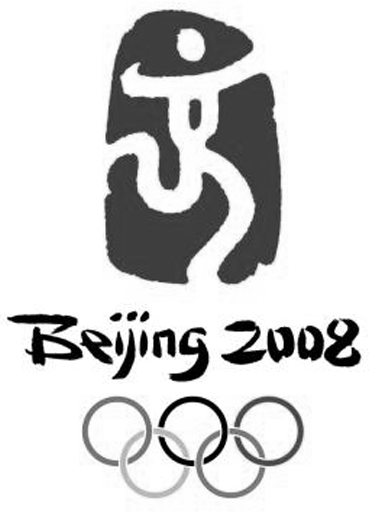
\includegraphics[width=5cm]{beijing.png}
    \item[2024 年巴黎奥运会] 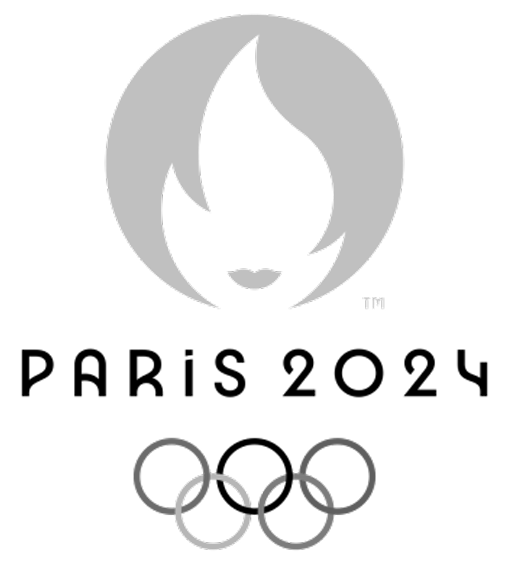
\includegraphics[width=5cm]{paris.png}
  \end{multifigures}

  \circlednumber{1} 文化是物质文明和精神文明繁荣的表现

  \circlednumber{2} 继承和发扬中华优秀传统文化,需要实现中华优秀传统文化创新性发展

  \circlednumber{3} 文化多样性是实现世界文化繁荣的必然要求

  \circlednumber{4} 任何一种文化都是对当下时代精神的展现

  \begin{choices}
  \item \circlednumber{1}\circlednumber{2}
  \item \circlednumber{1}\circlednumber{3}
  \item \circlednumber{2}\circlednumber{3}
  \item \circlednumber{3}\circlednumber{4}
  \end{choices}
\end{question}

\needspace{3\baselineskip}
\begin{question}
  2025 年 1 月 6 日,美国国会参众两院举行联席会议,依次递交第 60 届美国总统选举来自各州及华盛顿特区的选举人票投票结果,由两名参议员和两名众议员轮流唱票。结果显示,特朗普获得 312 张选举人票,超过赢得总统选举所需的 270 票,正式确认前总统、共和党总统候选人特朗普当选为美国总统。由此可见

  \circlednumber{1} 美国国会参众两院拥有最高行政权力

  \circlednumber{2} 美国总统由选民选举产生、对选民负责

  \circlednumber{3} 美国的代议制政体维护了选民的政治权利

  \circlednumber{4} 代议制是现代民主政体的共同特征

  \begin{choices}
  \item \circlednumber{1}\circlednumber{2}
  \item \circlednumber{1}\circlednumber{3}
  \item \circlednumber{2}\circlednumber{3}
  \item \circlednumber{2}\circlednumber{4}
  \end{choices}
\end{question}

\needspace{3\baselineskip}
\begin{question}
  孙某 1999 年生,因先天性疾病导致其智力远低于同龄人。2018 年从特殊教育学校毕业后,在家附近的小超市当搬运工维持生活。由此可见

  \circlednumber{1} 孙某有权通过劳动获得收入维持自身生活

  \circlednumber{2} 国家设立专门教育机构保障特殊群体受教育权

  \circlednumber{3} 孙某患有严重残疾,是无民事行为能力人

  \circlednumber{4} 孙某接受慈善企业的爱心捐款,须经其监护人同意或追认

  \begin{choices}
  \item \circlednumber{1}\circlednumber{2}
  \item \circlednumber{1}\circlednumber{3}
  \item \circlednumber{2}\circlednumber{3}
  \item \circlednumber{3}\circlednumber{4}
  \end{choices}
\end{question}

\needspace{3\baselineskip}
\begin{question}
  某学校在学生家庭情况调查中发现,本校学生小王因父母离异长期跟随父亲生活。小王父亲王某长期酗酒后对小王实施家庭暴力、长期侵占小王母亲支付的抚养费。该校有关负责人多次劝说无果后,决定报告公安机关并对王某提起诉讼。可能的结果有

  \circlednumber{1} 公安机关发布对小王的人身安全保护令

  \circlednumber{2} 人民法院判决王某失去小王的监护权

  \circlednumber{3} 人民检察院对王某的家庭暴力行为继续追究刑事责任

  \circlednumber{4} 民政部门解除小王与王某的父母子女关系

  \begin{choices}
  \item \circlednumber{1}\circlednumber{2}
  \item \circlednumber{1}\circlednumber{4}
  \item \circlednumber{2}\circlednumber{3}
  \item \circlednumber{2}\circlednumber{4}
  \end{choices}
\end{question}

\needspace{3\baselineskip}
\begin{question}
  姜某和林某 2004 年生,从小青梅竹马。2024 年年末两人决定于 2025 年元旦当天办理结婚登记,且约定婚前个人的一切财产都属于夫妻共同财产。姜某父亲早年因公殉职,生前给妻子和姜某留下存款 20 万元。林某名下有一套位于某市繁华地段的商铺出租,每月可获得租金收入 2800 元。下列说法正确的是

  \circlednumber{1} 根据约定,姜某分得的财产 10 万元和林某名下的商铺均属于夫妻共同财产

  \circlednumber{2} 办理结婚登记前,两人的财产均为独立享有

  \circlednumber{3} 姜某母亲独立承担抚养义务,占有 20 万元遗产的大部分继承权

  \circlednumber{4} 若两人最终离婚,商铺依然属于共同财产

  \begin{choices}
  \item \circlednumber{1}\circlednumber{2}
  \item \circlednumber{1}\circlednumber{4}
  \item \circlednumber{2}\circlednumber{3}
  \item \circlednumber{2}\circlednumber{4}
  \end{choices}
\end{question}

\needspace{3\baselineskip}
\begin{question}
  当一个主体的积极和消极两个方面同时出现在一个人的头脑中时,可能会也可能不会被体验为心理上的不愉快。这种不舒服的心理也被称为认知失调,会导致逃避、拖延,甚至故意尝试极端以解决这种心理。由此可见

  \circlednumber{1} 逻辑思维遵循同一律的准则,事物的两方面最终趋于统一和确定

  \circlednumber{2} 逻辑思维遵循矛盾律的准则,事物的两方面不能互相反对

  \circlednumber{3} 人的思维来源于实践,正确的思维认识只能来源于实践

  \circlednumber{4} 学习科学思维,必须坚持求真务实

  \begin{choices}
  \item \circlednumber{1}\circlednumber{2}
  \item \circlednumber{1}\circlednumber{3}
  \item \circlednumber{2}\circlednumber{3}
  \item \circlednumber{3}\circlednumber{4}
  \end{choices}
\end{question}

\needspace{3\baselineskip}
\begin{question}
  化学上称只含有两种元素且元素之一为氧的化合物为氧化物。如果一种氧化物与碱反应只生成盐和水,则是酸性氧化物;如果一种氧化物与酸反应只生成盐和水,则是碱性氧化物;如果一种氧化物无论与酸或与碱反应均能生成盐和水,则是两性氧化物。酸性氧化物中大多数是非金属氧化物,非金属氧化物中大多数是酸性氧化物。下列推论正确的是

  \circlednumber{1} 两性氧化物的断定方法属于联言判断

  \circlednumber{2} 存在既非酸性氧化物也非金属氧化物的氧化物

  \circlednumber{3} 酸性氧化物与碱性氧化物的概念外延属于矛盾关系

  \circlednumber{4} 能与一种氧化物反应生成盐和水的物质必然是酸或碱

  \begin{choices}
  \item \circlednumber{1}\circlednumber{2}
  \item \circlednumber{1}\circlednumber{3}
  \item \circlednumber{2}\circlednumber{3}
  \item \circlednumber{2}\circlednumber{4}
  \end{choices}
\end{question}

\needspace{4\baselineskip}
\begin{flushleft}
  {\bfseries 二、非选择题:本题共 4 小题,共 52 分。}
\end{flushleft}

\needspace{3\baselineskip}
\begin{question}
  阅读材料,完成下列要求。

  \begin{kaiti-indented}
    1 月 9 日,陕西省十四届人大常委会第十四次会议在西安闭幕。会议表决通过了《黄帝陵保护条例》、《实施家庭教育促进法办法》和《陕西省法律援助条例》,表决通过了省人大常委会工作报告稿,根据表决结果决定任命李九红为陕西省副省长。

    完成各项议程后,中共陕西省委书记、省人大常委会主任赵一德作了讲话。他强调,全省各级人大及其常委会要深入学习贯彻中央经济工作会议精神和习近平总书记近期一系列重要讲话重要指示精神,认真落实省委经济工作会议部署,主动适应进一步全面深化改革和经济社会发展需要,扎实做好立法、监督、决定、任免等各项工作,紧扣打造“四个机关”强化自身建设,为高质量完成“十四五”规划目标任务、奋力谱写中国式现代化建设的陕西新篇章贡献人大力量。
  \end{kaiti-indented}

  结合材料,运用《中国特色社会主义》《政治与法治》知识,分析陕西省人大常委会在坚持人民当家作主、党的领导、依法治国有机统一中发挥的作用。(11 分)
\end{question}

\needspace{3\baselineskip}
\begin{question}
  阅读材料,完成下列要求。

  \begin{kaiti-indented}
    近日,中共中央、国务院印发《关于深化养老服务改革发展的意见》,围绕加快建设符合我国国情的养老服务体系,优化基本养老服务供给,提出一揽子政策举措。

    首次提出加快健全覆盖城乡的县乡村三级养老服务网络。根据《意见》部署,养老服务网络到2029年基本建成,到2035年更加健全。通过持续推进建设,把养老服务网织得更密更牢,稳稳兜住老年人的养老服务需求。

    以推动三类养老服务贯通协调为改革重点,明确各类养老服务功能作用。加强各类养老服务在老年人需求场景的协调联动,让老年人在家庭、社区、机构都能享受方便可及的服务。

    要大力发展银发经济,释放养老消费潜力。从消费趋势看,老年人与年轻人消费边界不断融合,消费观念、消费结构愈发重合,更加注重个性化和悦己消费,成为消费多元化发展的关键群体;从产业发展看,银发经济促使各产业为老年人创新、创造更多的服务产品,涉及老年人生活的方方面面,为老年人服务注入了新的动力。
  \end{kaiti-indented}

  (1)结合材料,运用《经济与社会》知识,阐述如何进一步建设养老服务体系。(9 分)

  (2)结合材料,运用《哲学与文化》知识,对“银发产业经济效益弱,当前暂无必要大力发展”这一观点予以评价。(7 分)
\end{question}

\needspace{3\baselineskip}
\begin{question}
  阅读材料,完成下列要求。

  \begin{kaiti-indented}
    钱某是某县的一位知名女企业家。1997 年 5 月,钱某与孙某经亲戚介绍相识并决定结婚,孙某父母以价值 400 万元的一套独栋别墅作为彩礼赠与夫妻双方。婚礼时,孙某未达到规定的男性结婚年龄,后拖延到 1999 年 10 月才补办了结婚登记。1998 年 11 月,钱某的长子孙某甲出生。2004 年 1 月,次子孙某乙出生。2007 年 7 月,女儿孙某丙出生。钱某和孙某长期异地生活从事经商,2009 年 10 月,钱某因生意失败,欠下债务 300 万元并以此别墅作为抵押,约定分 15 年还清。2023 年,钱某病重,后经治疗无效逝世。清点钱某个人物品时,孙某发现钱某与情夫王某在外长期同居,还在 2012 年生育一女小王,并每月秘密向小王汇款抚养费 3000 元。债主要求支付 2023 年所欠分期款项时,孙某以不知情为由拒绝支付。2025 年 1 月,孙某因车祸不幸逝世,获得肇事车主 85 万元赔偿。
  \end{kaiti-indented}

  根据材料,运用《法律与生活》知识,对本题中所有继承权、债权、抚养权进行合理配置。(15 分)
\end{question}

\needspace{3\baselineskip}
\begin{question}
  阅读材料,完成下列要求。

  \begin{kaiti-indented}
    日本出租车行业破产数量正在急剧增加。日本帝国数据库网日前发布的数据显示,2024 年日本国内发生的出租车公司倒闭清算 35 件,停业、解散 47 件,共计 82 家出租车公司选择退出市场,与 2023 年 全年 63 件相比增加 19 件、增长了 30.2\%,超过了 2019 年的 73 件,创历史新高。报告称,在 2024 年出租车行业的 35 起破产中,至少四成以上的主要原因是司机等人手不足。出租车司机短缺情况日益严重,以及因人手不足而带来的出租车车辆剩余,进而导致车辆运转率下降,给各家出租车公司运营造成严重影响。日本国土交通省数据显示,截至 2023 年 3 月底,日本全国在出租车公司工作的司机约为 22 万人,与疫情前 2019 年 3 月相比减少了约两成。相比之下,法人出租车保有车辆的减少幅度不足10\%,司机减少速度远超车辆数量的下降。供需错配进一步加重了行业困境。此外,出租车主要燃料价格的持续高涨也对出租车企业造成了沉重负担。日本液化石油气价格飞涨,能源成本增加,经营压力显著加剧,也是导致出租车运营商放弃业务数量增加的一个因素。
  \end{kaiti-indented}

  根据材料,运用《逻辑与思维》知识,运用科学思维说明中国出租车行业可以吸取的行
  业经验和做法,并说明所使用的科学思维方法。(10 分)
\end{question}

\end{document}
